% RECOVERED PARTIAL 20260708
% Reconstructed from Codex log sed/nl fragments.
% Gaps below mark original line ranges not present in recovered logs.

% =====================================================================
% Experimental Astronomy / Springer Nature layout.
% Uses the official Springer Nature sn-jnl.cls template package.
% Compile with pdfLaTeX for Springer submission-system compatibility.
% =====================================================================
\documentclass[pdflatex,sn-mathphys-num]{sn-jnl}
\usepackage{amsmath,amssymb,amsfonts}
\usepackage{booktabs}
\usepackage{graphicx}
\usepackage[section]{placeins}
\renewcommand{\topfraction}{0.92}
\renewcommand{\bottomfraction}{0.8}
\renewcommand{\textfraction}{0.07}
\renewcommand{\floatpagefraction}{0.75}
\usepackage{xcolor}
\usepackage{tikz}
\usetikzlibrary{arrows.meta,positioning}
\setlength{\emergencystretch}{3em}
\newcommand{\keV}{\,\mathrm{keV}}
\newcommand{\MeV}{\,\mathrm{MeV}}
\newcommand{\cms}{\,\mathrm{cm^{-2}\,s^{-1}}}
\newcommand{\phcms}{\,\mathrm{ph\,cm^{-2}\,s^{-1}}}
\newcommand{\cps}{\,\mathrm{s^{-1}}}
\newcommand{\wii}{W_{511}}
\newcommand{\aeff}{A_{\mathrm{eff}}}
\newcommand{\fzero}{F_{0}}
\newcommand{\fthree}{F_{3\sigma}}
\newcommand{\added}[1]{{#1}}
\newcommand{\rewritten}[1]{{#1}}
\raggedbottom

\begin{document}

\title[Detector-coupled Monte Carlo estimate for a balloon-borne 511 keV TES telescope]{Detector-coupled Monte Carlo estimate of background and unresolved-line sensitivity for a balloon-borne 511 keV Laue-lens TES telescope}

\author*[1]{\fnm{Authors} \sur{omitted for review}}

\affil*[1]{\orgname{Affiliations omitted for review}}

\abstract{The Galactic 511 keV annihilation signal is dominated by diffuse bulge and disk emission, while compact or point-like contributions remain poorly constrained. We present a detector-coupled Monte Carlo estimate for a balloon-borne pointed telescope combining a 10 m Ge(111) Laue lens with a transition-edge sensor microcalorimeter focal plane. The signal chain transports focused 511 keV photons through the Be aperture into the detector/cryostat mass model. The background chain transports prompt atmospheric particles and photons and production-position-sampled delayed activation decays through the same model. Prompt, delayed, and signal streams are analyzed with a common $510.58$--$511.42\keV$ window, CsI anticoincidence veto, and topology/field-of-view consistency selection. For a reference point-source flux of $10^{-4}\phcms$, the selected day-15 signal and background rates are $1.19\times10^{-3}\cps$ and $3.92\times10^{-2}\cps$, respectively; prompt atmospheric events account for 93.4\% of the selected background. Folding these rates through the adopted synthetic 20 d trajectory gives $Z_{20\mathrm{d}}=7.80$ and a corresponding $3\sigma$ flux threshold of $3.85\times10^{-5}\phcms$. The result is a selected-rate flight-sensitivity estimate for a spectrally unresolved compact 511 keV source under the reference geometry and response model. Prompt atmospheric events dominate the selected background, while the delayed component is smaller but materially structured, identifying shielding, side-entry collimation, local materials, and activation validation as the main next engineering and analysis targets.}

\keywords{Gamma-ray instrumentation, 511 keV annihilation line, transition-edge sensors, Laue lens, balloon-borne telescope, activation background}

\maketitle

\section{Introduction}
\label{sec:intro}

The 511 keV annihilation emission from the Galactic-center region is a key observational window on the origin of Galactic positrons. Spectroscopically, it consists of a two-photon line near 511 keV and a positronium continuum on its low-energy side: direct electron--positron annihilation, or para-positronium decay, produces two photons near 511 keV, whereas ortho-positronium decay produces a three-photon continuum. After slowing in the interstellar medium, positrons form positronium or annihilate directly, so the line strength, line profile, and positronium continuum together encode the annihilation medium \cite{Prantzos2011,Jean2006}. Observations led by INTEGRAL/SPI measure the total Galactic 511 keV flux; in approximate steady state, this flux corresponds to a positron annihilation rate of order a few $\times10^{43}\,\mathrm{e^+\,s^{-1}}$ \cite{Prantzos2011,Kierans2020}. This scale links Galactic-center spectroscopy to the Galaxy-wide positron-supply problem: candidate supply channels include $\beta^+$ radioactive nuclei synthesized in stellar explosions, pair-producing compact objects, and non-standard particle processes, but present data do not uniquely identify which class dominates \cite{Prantzos2011,Siegert2016AA}.

Past wide-field observations have established the diffuse morphology of this emission. INTEGRAL/SPI reveals a bright central bulge together with a fainter Galactic disk, and a 20-year analysis recovers central, broad-bulge, and disk structures while finding only marginal evidence for additional associations \cite{Siegert2016AA,Yoneda2025}. The 2016 COSI balloon flight independently detected the bulge signal and found indications of emission more extended than a point source \cite{Kierans2020,Siegert2020COSI}. Spectroscopy also constrains the physical state and kinematics of the annihilation medium: the SPI line resolves into a narrow component of $\sim 1.3\keV$ FWHM and a broader $\sim 5.4\keV$ component, and centroid and width variations have been searched for across the inner Galaxy \cite{Jean2006,Siegert2019Kinematics}. Nevertheless, the 511 keV sky records where positrons annihilate after slowing, not necessarily where they were first produced; before thermalization, positrons can propagate through the magnetized, multiphase interstellar medium. Existing diffuse-morphology and spectroscopy constraints therefore do not by themselves identify the dominant source class or reconstruct the transport history before annihilation \cite{Prantzos2011}.

This motivates narrow-field, high-resolution pointed observations. Wide-field Compton and coded-mask instruments are well suited to measuring the overall diffuse bulge and disk, and they can also be searched for point sources; however, a complementary technique is needed to test whether the central region contains an unresolved central enhancement, point sources, or measurable line-kinematic structure. Detecting a point-like or narrowly concentrated 511 keV feature would show that some annihilation is spatially localized; a non-detection would instead limit the compact component without excluding source populations whose positrons escape and annihilate diffusely. Compact-source searches based on INTEGRAL/IBIS coded-mask data have found no Galactic 511 keV point sources and give a $2\sigma$ point-source upper limit of about $1.6\times10^{-4}\phcms$ for a $\sim 10$ Ms Galactic-center exposure \cite{DeCesare2011}. This non-detection limit sets the flux scale reached by existing compact-source searches and provides a comparison target for new narrow-field 511 keV pointing instruments.

Laue optics provide one route to such pointed observations by using Bragg diffraction in transmission to concentrate photons from a known direction onto a small focal plane \cite{Barriere2009Laue,Barriere2011LauePrototype}. By decoupling collecting area from active detector area, focusing can improve point-source sensitivity whenever detector-associated background dominates \cite{Weidenspointner2006MAX}. A compatible focal plane must combine a narrow energy response with adequate 511 keV detection efficiency. Transition-edge sensor (TES) microcalorimeters read the deposited energy in $\gamma$-ray absorbers with superconducting transition thermometers and can provide sub-keV energy resolution at 511 keV \cite{Shirazi2023}. Arranging TES microcalorimeters in arrays gives the active area needed to cover the focused spot, while thick absorbers and multiple absorber layers increase the interaction probability for 511 keV photons. The Laue-optics/TES-array combination therefore concentrates the incident phase space while preserving high spectral discrimination: the optics focus photons from the target direction onto a small focal plane, and, for the unresolved 511 keV line considered here, the TES response makes a narrow line-window cut a useful background-rejection tool. The combination trades sky coverage for a concentrated beam and high-resolution spectroscopy, making it complementary to wide-field measurements of the bulge and disk rather than a replacement for them. Continuum studies or broader astrophysical line profiles would require the corresponding energy band, optical configuration, and background model, and therefore a different sensitivity definition.

In practice, focusing and a narrow line window do not by themselves determine the achievable sensitivity, because MeV line instruments are often limited by local instrumental backgrounds. Spaceborne and balloon-borne instruments alike can suffer activation products, local annihilation radiation, and continuum backgrounds induced by cosmic rays and secondary particles \cite{Sturner2003,Gehrels1985}. For a balloon payload, the residual atmosphere also provides a strong photon and particle field that varies with altitude, latitude, and geomagnetic cutoff; in the present 511 keV case, atmospheric photons and particles can directly produce prompt detector events and secondary annihilation radiation, and can also generate radioactive nuclei in the detector, shield, and surrounding structure whose decays form a time-dependent delayed component. Because the celestial signal sits at the same energy as atmospheric and instrumental annihilation features, sensitivity cannot be inferred from the lens effective area and detector energy resolution alone; it also depends on the surrounding mass distribution, the active shielding and event selection, the radiation environment, and the accuracy with which the residual background is modeled. Recent bottom-up simulations of the 2016 COSI balloon flight illustrate the level of payload and detector-response modeling---including activation lines and anticoincidence response---needed to validate such a background estimate against flight and calibration data \cite{Gallego2025Balloon,Beechert2022,Ciabattoni2025ACS}.

In this work we develop an end-to-end detector-coupled Monte Carlo chain for this concept and use it to estimate the in-flight background and point-source performance at balloon altitude and to provide directional guidance for design optimization. The chain takes the EXPACS/PARMA atmospheric cosmic-ray field as input and, at balloon altitude, transports the prompt particles while tracking their activation products, yielding both the prompt atmospheric background and the delayed activation background that builds up over the flight; the focused 511 keV reference signal is provided by a 10 m Ge(111) Laue-optics model. The signal and both backgrounds are injected into the same representative balloon-borne TES focal-plane mass model (a dilution-refrigerator cold end, passive shielding, and an active anticoincidence shield), processed with a common narrow energy window, anticoincidence veto, and topology/field-of-view selection, and folded along a reference flight trajectory to give the selected signal rate, the background composition, and the counting significance. The selected background is dominated by the prompt atmospheric component, so the shield geometry, side-entry collimation, and shield material are the most direct directions for design optimization; the delayed activation and the upstream optics-hardware background enter the same evaluation as secondary components. This work thereby estimates the in-flight background and detection performance of the balloon platform and indicates directions for design optimization.

\subsection{Science and instrument requirements}
\label{sec:requirements}

The simulated instrument is aimed at 511 keV point-source or unresolved-central-excess components from the Galactic-center region that have not been detected by previous instruments. Existing INTEGRAL/SPI measurements have established a 511 keV sky dominated by diffuse bulge and disk emission and limit point-like 511 keV sources superposed on that diffuse emission to fluxes of order $10^{-4}\phcms$; an independent INTEGRAL/IBIS compact-source search also found no Galactic 511 keV point sources and gives an upper limit of about $1.6\times10^{-4}\phcms$ for a $\sim10$ Ms Galactic-center exposure \cite{Knodlseder2005AllSky,DeCesare2011}. For a representative 511 keV atmospheric transmission of $T\simeq0.739$ at balloon altitude, this limit corresponds to an above-payload photon-flux scale of about $1.2\times10^{-4}\phcms$. The simulation therefore adopts $\fzero=10^{-4}\phcms$ as the reference point-source photon-flux scale. Compared with the wide-field spectroscopic and coded-mask searches performed by INTEGRAL, the modeled payload adds Laue focusing to improve the point-source response and uses a high-energy-resolution, multilayer thick-absorber TES microcalorimeter array as the focal-plane detector to sharpen the 511 keV line measurement \cite{Shirazi2023,Caputo2017}.

This work first considers a balloon payload as an early test platform, with the expectation that the approach can later be extended to a satellite observing platform.

This goal imposes four requirements on the instrument and the simulation: first, the telescope must concentrate 511 keV photons onto a small focal plane, so that detector-associated background is reduced without sacrificing collecting area. Second, the focal-plane response must support a sub-keV energy window, so that the line-window background scales with a narrow spectral interval rather than a broad MeV-band continuum. Third, the detector and shield model must suppress atmospheric, activation, and side-entry backgrounds while explicitly accounting for the passive material near the TES absorbers. Fourth, the simulation chain must treat prompt background, delayed activation, focused signal, vetoes, event topology, and mission-time variation consistently, so that signal and background are evaluated under the same detector selection.

The remainder of this paper is organized as follows. Section~\ref{sec:geometry} describes the detector and cryostat mass model; Section~\ref{sec:framework} the simulation framework---the workflow, optics coupling, background sources, event selection, and mission-time fold; Section~\ref{sec:results} the selected-rate and sensitivity results together with the normalization, convergence, and boundary checks; and Section~\ref{sec:discussion} the discussion and conclusions.

\section{Detector and cryostat mass model}
\label{sec:geometry}

The detector mass model is an engineering Geant4/MEGAlib proxy mass model that contains a balloon-borne multilayer TES array mounted at the cold end of a compact dilution refrigerator (DR) \cite{Shirazi2023,Gottardi2021TESReview}. The detector model also contains typical DR cryostat structures, active shielding, passive shielding, magnetic shielding, side-entry windows, collimation structures, copper thermal structures, and other cryogenic service-mass proxies. Figure~\ref{fig:mass_model} shows two-dimensional views of the mass model used in this paper.

The TES detector concept uses an absorber-coupled AlMn film structure developed in our laboratory; the advantages of AlMn alloy include transition-temperature tunability through composition and annealing, suitability for array fabrication, and relatively low magnetic-field sensitivity \cite{Xie2026AlMn,Vavagiakis2017AlMnMagnetic}. In the present concept, the TES thermometer film is an AlMn film of order $200\,\mathrm{nm}$ thickness, whereas the $\gamma$-ray absorber is a millimetre-scale metal body. The absorber uses $1.5\times1.5\times3.0\,\mathrm{mm^3}$ Ta pixels; the high atomic number of Ta increases the interaction probability for 511 keV photons, and a $3.0\,\mathrm{mm}$ thickness corresponds to about a $49\%$ single-layer interaction probability at 511 keV, so the six-layer array can provide a near-unity geometric interaction probability. In the current geometry, the center-to-center spacing between adjacent Ta array layers is $12\,\mathrm{mm}$; this spacing is used to preserve the multilayer hit topology required for the Compton-kinematic veto discussed below. The choice of Ta also considers that this volume can provide a sufficiently high saturation energy, low low-temperature specific heat (this paper uses an order-of-magnitude estimate of $10^{-2}\,\mathrm{J\,K^{-1}\,m^{-3}}$), and a relatively high photoelectric-to-Compton interaction ratio; based on NIST XCOM cross sections near 511 keV, this ratio is about 0.731 \cite{NISTXCOM}. Based on laboratory experience and by substituting the current Ta absorber heat capacity of $67.5\,\mathrm{pJ/K}$, the simulation adopts $\Delta E_{\mathrm{FWHM}}\simeq420\,\mathrm{eV}$ at 511 keV as the current simulated energy resolution.

Because the TES film and Ta absorber differ greatly in size and mass, and because the TES film itself does not contribute significant 511 keV interactions, the transport geometry uses the Ta absorber to represent the main sensitive volume of a TES pixel. The explicit sensitive volume has six layers, 376 Ta absorber pixels per layer, and 2256 pixels in total, with 1.5 mm length and width and 3 mm thickness. A Si substrate proxy is placed below each Ta pixel, using Si to represent the substrate; this also preserves the elastic-scattering contribution that silicon may provide in neutron transport. TES-film, wiring, and readout details are not built layer by layer as explicit interaction volumes; instead, they enter the model through the assumed energy response and service-mass proxies. In the current manuscript, the TES energy resolution is used as the 511 keV line-window width, with W511 = 511 keV $\pm$ 420 eV, i.e. 510.58--511.42 keV.

The TES array is mounted on the required copper support and thermal-link structures. Copper provides the decisive thermal-conduction path; a copper thermal finger exits through the bottom hole of the sample box and connects to the 50 mK cold plate. The near-field TES sample box serves as both magnetic shielding and local passive shielding. The current mainline geometry consists of a 2 mm Nb inner layer and a 2 mm MuMetal outer layer, with MuMetal represented in the material table as Ni:Fe = 4:1. The sample-box entrance window is covered by a thin Al window; the rear end cap retains the hole for the cold finger. A W--Nb double-layer sample box is treated as a comparison passive-shielding + magnetic-shielding material design; the X-ray window is opened on the side of the cryostat, with a 300 $\mu$m thick Al window embedded in the thermal-shield shell inside each cryostat layer, a 25 $\mu$m thick Be window placed in the vacuum shell, and an $x$-thick W collimator placed outside the Be window, with the collimator opening strictly aligned to the TES pixels. The side window is strictly defined through Boolean operations. The mass model also introduces scintillator active shielding, wrapped around the outer side wall, bottom, and top of the cryostat. Segmented CsI active shielding is used, with a radial side-shield thickness of 4 cm; the bottom and top shields are included in the geometry as axial end volumes. CsI volumes enter the simulation as transport and activation materials, and their deposited energies are read in post-processing to apply the active veto; the counting threshold is 50 keV. BGO active shielding is treated as a material-comparison case; the BGO threshold is 70 keV. Considering the physical layout of the DR and the side-entry optical path, the cryostat instrument frame is rotated as a whole by 45 degrees, so that the local side window is tilted $45^\circ$ upward in the zenith-frame source coordinates.

\begin{figure}[t]
\centering

\includegraphics[width=0.62\linewidth]{paper_source_figure_table/fig_mass_model_xz_overview.png}
\caption{Two-dimensional overview of the detector/cryostat proxy mass model, showing the X--Z view of the DR tower, detector bay, active shield, and 511 keV side-entry beam path.}
\label{fig:mass_model}
\end{figure}

\FloatBarrier

\section{Simulation framework}
\label{sec:framework}

This section describes the whole simulation chain from source construction to flight-performance assessment. The focused signal and detector background start from two mass models. The focused-signal branch is implemented in the Laue-optics model 10m upstream, focusing 511 keV photons onto the focal plane, \textcolor{red}{also considering the influence of the instantaneous background and activation background on this mass model}, and outputting the focal-plane slice together as the focused signal. The detector-background branch directly simulates, in the detector/cryostat mass model of Section 2, the delayed background caused by prompt atmospheric cosmic rays and activated nuclides. The prompt atmospheric cosmic rays all use the far-field definition defined by megalib, according to the zenith-angle flux output by the expacs library, with full-solid-angle input. For activated nuclides, the real positions where nuclides are produced are recorded, and then activation background is generated by sampling according to the production rate. The focused signal, instantaneous background, and activation background are normalized and superposed to build the total spectrum. After detector response, anticoincidence, and event selection based on Compton tracks inverted from different pixels, the effective spectrum is used for post-processing statistical analysis and flight-performance assessment.

The above simulation is for a specific balloon-flight moment, longitude and latitude, and altitude. Although for an observation time such as one hour equivalent to several Monte Carlo events, this position can be regarded as constant. However, for a long-time flight on the scale of days, the altitude, longitude, and latitude obviously change significantly. This causes changes in the magnetic-rigidity cutoff for instantaneous cosmic rays and changes in the atmospheric transmission for the signal, and the activation background itself also changes with the incident cosmic-ray flux and different stages of the decay chain. This reminds us that the background-signal at a reference moment should not be linearly extrapolated in time to evaluate the time-folded flight performance over the whole working time. Therefore, we introduce a reasonable analytical flight-trajectory--time curve to evaluate the performance over the whole working cycle, and simulate multiple points on the curve to verify the rationality of the curve.

\begin{figure}[t]
\centering
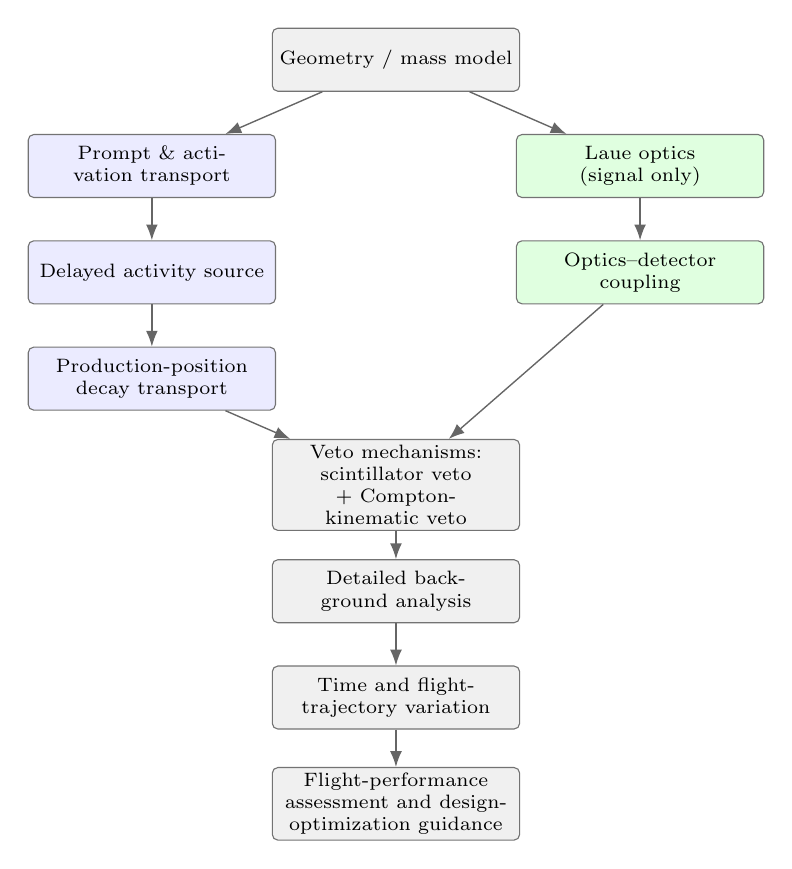
\begin{tikzpicture}[
  box/.style={rectangle, rounded corners=2pt, draw=black!55, line width=0.4pt,
              align=center, font=\scriptsize, text width=30mm, minimum height=8mm, inner sep=2pt},
  bg/.style={box, fill=blue!8},
  sig/.style={box, fill=green!12},
  shr/.style={box, fill=black!6},
  flow/.style={-{Latex[length=2mm]}, draw=black!60, line width=0.5pt}
]
\node[shr] (geo)    at (0,0)        {Geometry / mass model};
\node[bg]  (prompt) at (-3.1,-1.35) {Prompt \& activation transport};
\node[bg]  (delay)  at (-3.1,-2.7)  {Delayed activity source};
\node[bg]  (decay)  at (-3.1,-4.05) {Production-position decay transport};
\node[sig] (optics) at (3.1,-1.35)  {Laue optics (signal only)};
\node[sig] (couple) at (3.1,-2.7)   {Optics--detector coupling};
\node[shr] (sel)    at (0,-5.4)     {Veto mechanisms: scintillator veto $+$ Compton-kinematic veto};
\node[shr] (detail) at (0,-6.75)    {Detailed background analysis};
\node[shr] (fold)   at (0,-8.1)     {Time and flight-trajectory variation};
\node[shr] (out)    at (0,-9.45)    {Flight-performance assessment and design-optimization guidance};
\draw[flow] (geo) -- (prompt);
\draw[flow] (geo) -- (optics);
\draw[flow] (prompt) -- (delay);
\draw[flow] (delay) -- (decay);
\draw[flow] (optics) -- (couple);
\draw[flow] (decay) -- (sel);
\draw[flow] (couple) -- (sel);
\draw[flow] (sel) -- (detail);
\draw[flow] (detail) -- (fold);
\draw[flow] (fold) -- (out);
\end{tikzpicture}
\caption{Simulation chain used in this work. Blue nodes are the prompt and
delayed background streams, green nodes the focused-signal optics, and grey
nodes the shared geometry, veto mechanisms, detailed background analysis,
time/trajectory variation, and final flight-performance assessment. The focused
signal and all background streams are evaluated under the same detector response
and veto definitions before background decomposition, mission-time variation,
and design-optimization judgments are made.}
\label{fig:workflow}
\end{figure}

\FloatBarrier

\subsection{Laue optics and detector-coupled signal replay}
\label{sec:optics}

This simulation adopts a laue-lens system based on mosaic Ge(111) crystals \cite{Barriere2009Laue,Barriere2011LauePrototype}. Through optical design, it realizes a 10 m focal length, \textcolor{red}{a multi-ring system realizes the 450keV-550keV detection band}, and an effective area of 20cm**2 at 511keV; the effective area is calculated as
\begin{equation}
  A_{\mathrm{eff}}(E)=A_{\mathrm{inc}}\frac{N_{\mathrm{fp}}(E)}{N_{\mathrm{inc}}(E)}
  \label{eq:laue_aeff}
\end{equation}
where $A_{\mathrm{inc}}$ is the Monte Carlo incident sampling area, $N_{\mathrm{inc}}(E)$ is the number of incident photons, and $N_{\mathrm{fp}}(E)$ is the number of photons satisfying the focusing/focal-plane interception condition.
The mosaic system is adopted to make the Monte Carlo calculation convenient while satisfying the expected focusing performance; other candidate schemes are also possible for actual engineering adaptation.

In this simulation, the laue optical branch gives the focusing-performance simulation and \textcolor{red}{also realizes particle transport of itself as mass}.

For this purpose, the diffraction probability of photons by the crystal is no longer superposed onto photons as an efficiency parameter, but is defined as a discrete process at the Geant4 application layer \cite{Agostinelli2003,Allison2016}. The process takes the diffraction probability $R(|\Delta\theta|)$ according to the angular deviation of the current photon relative to the crystal plane, and converts it into a finite equivalent diffraction mean free path $\lambda_{\mathrm{diff}}$, so that the accumulated diffraction probability when the photon crosses a crystal path $\ell$ reproduces this value: $1-\exp(-\ell/\lambda_{\mathrm{diff}})=R(|\Delta\theta|)$, namely $\lambda_{\mathrm{diff}}=-\,\ell/\ln[1-R(|\Delta\theta|)]$; to avoid double counting with standard photoelectric absorption, $R$ is first normalized by the unabsorbed fraction ($R/(1-A)$) and then converted into a mean free path. After this mean free path is returned to Geant4, the diffraction process and the standard electromagnetic processes (photoelectric absorption and Compton scattering) each sample interaction lengths in the same competition framework, and the shortest one decides which process occurs first, rather than forcibly intercepting photons at the crystal boundary. Photons not selected to undergo diffraction still continue transport according to the standard electromagnetic physics, and may be absorbed, scattered, or directly transmitted.

The diffraction probability is preferentially given by interpolation in an external XOP/CRYSTAL rocking-curve map as a function of angular deviation: this curve is calculated offline once in the preprocessing stage by the CRYSTAL/diff\_pat module of the XOP toolkit (called through xoppylib, with DABAX crystallographic data as input) \cite{SanchezDelRio2011XOP}, and gives the Ge(111) reflectivity/transmissivity/absorption curves as a function of angular deviation; during transport, the angular deviation is calculated in real time for every step inside the crystal, and the current diffraction probability is obtained by interpolation on that curve, namely ``offline library tabulation, probability used by angle during transport''. The mosaic orientation is implemented by applying a Gaussian angular perturbation to the ideal Bragg-plane normal, with the perturbation width given by the 30 arcsec mosaic FWHM; after diffraction occurs, the outgoing direction is mirror-reflected according to the perturbed plane normal, and the photon energy is unchanged. This split in which the ``process class only handles the transport interface, and the independent model class handles probability and direction decisions'' follows the idea of existing crystal Bragg-reflection extensions in Geant4 \cite{Guan2023BraggReflection,Reiazi2025G4BraggReflection}, and extends it to the energy band needed here.

Here the signal photons use as reference the point source of the V404 source once detected by SPI \cite{Siegert2016V404}. V404 is a transient point source in the Galactic disk and is used here only as a reference. It is constructed using the megalib far-field source mode \cite{Zoglauer2006}; \textcolor{red}{the detailed construction method is given in Section 3.2.3 on point-source construction}. In addition to signal introduction, we also introduce the prompt cosmic-ray background component, also constructed in the far-field source mode, and introduce the activation-background construction. \textcolor{red}{The transport of the above three sources is simulated separately; in the three simulations, the particle flux, species, and energy crossing the plane where the focal plane is located are all intercepted as outputs; the three simulation outputs are normalized by equivalent observation time as the total output, and this total output can be separately input into the detector mass model as a parallel-beam source.}

\subsubsection{Reference point-source construction}
\label{subsec:pointsource}

The focused signal stream is defined by a reference astrophysical point
source. As a concrete example of the target class we take the 511\keV{}
emission episode of the microquasar V404 Cygni observed with INTEGRAL/SPI
\cite{Siegert2016V404}; V404 Cygni is a transient point source in the Galactic
disk and serves here only as a reference for the source class, not as a
predicted target flux. The reference flux scale itself,
$\fzero=10^{-4}\phcms$, is the above-atmosphere value motivated in
Section~\ref{sec:requirements}.

In the optics run, the source is a monochromatic 511\keV{} far-field beam:
photons arrive parallel to the optical axis, as from a point source at
astronomical distance, and are sampled uniformly over the incident aperture
$A_{\mathrm{inc}}$ of Eq.~(\ref{eq:laue_aeff}). Three independent seeds of
$5\times10^{4}$ primaries each give $1.5\times10^{5}$ transported photons, of
which 37,256 are diffracted and cross the focal plane; 37,194 of these
(99.8\%) fall within the $r=1.898\,\mathrm{cm}$ Be entrance window, with
focused-spot radii $r_{90}=1.03\,\mathrm{cm}$ and $r_{99}=1.25\,\mathrm{cm}$.
The within-window crossings form the event list that is replayed through the
Be aperture into the detector/cryostat model with the recorded positions and
directions.

The normalization ties this replay to the reference flux. At the detector
entrance the focused stream carries the rate
$\fzero\,\aeff(511\keV)\,T$, where $T=0.739$ is the reference 511\keV{}
atmospheric transmission at the day-15 trajectory anchor
(Section~\ref{sec:mission_time}); numerically this is
$1.48\times10^{-3}\cps$ at the reference flux. Equivalently, the generating
run corresponds to an observation time $N_{\mathrm{fp}}/[\fzero\,\aeff\,T]$,
and each replayed event carries the inverse of that exposure as its rate
weight; in the intermediate cut-flow bookkeeping of
Section~\ref{sec:selection} the same sample appears as a unit replay before
this scale is applied. After the common detector response and event selection,
the surviving signal rate is $1.19\times10^{-3}\cps$, corresponding to a
selected effective area of $S_{\wii}/\fzero=11.9\,\mathrm{cm^2}$. Because the
optics run contains only source photons, the replayed stream is signal-pure;
all backgrounds enter through the streams of Section~\ref{sec:background} and
the boundary terms of Section~\ref{subsec:upstream_optics_background}.

\subsection{Prompt atmospheric and delayed-activation source model}
\label{sec:background}

With the focused signal defined in Section~\ref{subsec:pointsource}, the
background side of the calculation requires two further source layers: the
prompt atmospheric field incident on the payload, and the delayed radioactive
population that this field builds up in the instrument. The two are
constructed separately, so that source generation does not absorb assumptions
that belong to detector selection: everything in this section defines incident
particles or decaying nuclei, while vetoes, topology cuts, and the hard line
window are applied only in Section~\ref{sec:selection}.

\subsubsection{Prompt atmospheric source}
\label{subsec:prompt_source}

The prompt atmospheric field is derived from EXPACS/PARMA. PARMA3.0 is an
analytical model parameterized from PHITS atmospheric-shower calculations and
benchmarked against terrestrial cosmic-ray measurements, and EXPACS is its
public tabulation and software interface
\cite{Sato2015EXPACS,Sato2016PARMA4}. PHITS supplies the underlying
particle-transport physics: primary cosmic rays interact with air nuclei, the
secondary hadrons, leptons, photons, and neutrons are transported through the
atmospheric column, and the resulting fluences are parameterized by altitude,
geomagnetic cutoff, solar modulation, energy, and direction. In this work
EXPACS/PARMA provides the differential incident flux as a function of particle
species, kinetic energy, zenith angle, geographic position, altitude, cutoff
rigidity, and solar activity, and is used only to construct the external
radiation fields; detector response, vetoing, topology selection, and
mission-time counting are applied downstream. The reference source definitions
use latitude $34^\circ$, longitude $100^\circ$, altitude $38\,\mathrm{km}$,
vertical cutoff rigidity $R_c=11.6\,\mathrm{GV}$, and the 2025-08-31 solar
condition corresponding to $W=118.3$.

The prompt source includes photons, neutrons, electrons, positrons, protons,
alpha particles, and negative and positive muons. For each particle family the
EXPACS/PARMA differential spectrum is converted into a MEGAlib far-field area
source covering the full zenith range $\theta=0^\circ$--$180^\circ$ and full
azimuth range $\phi=0^\circ$--$360^\circ$. The zenith dependence is represented
by 20 differential equal-$\mu$ angular bins, where $\mu=\cos\theta$ and each
bin subtends $\Delta\Omega=0.6283185307\,\mathrm{sr}$: the first ten bins cover
down-going particles, the last ten up-going or albedo-like particles. Both
hemispheres are retained in the prompt transport and in the
activation-production transport, so upward albedo particles are not discarded
at source construction. Figure~\ref{fig:expacs_fullsphere_flux} shows the
resulting full-sphere flux field.

\begin{figure}[t]
\centering

\includegraphics[width=\linewidth]{paper_source_figure_table/fig_expacs_fullsphere_flux.png}
\caption{EXPACS/PARMA full-sphere atmospheric flux field used to generate the prompt and activation-production transport inputs. Left: energy- and solid-angle-integrated fluxes for the eight transported particle families, separated into down-going and up-going hemispheres. Right: bin-integrated flux in the 20 equal-$\mu$ differential zenith bins used by the MEGAlib far-field source. The plot is generated from the source-definition inputs for latitude $34^\circ$, longitude $100^\circ$, altitude $38\,\mathrm{km}$, $R_c=11.6\,\mathrm{GV}$, and $W=118.3$.}
\label{fig:expacs_fullsphere_flux}
\end{figure}

The integrated source-plane fluxes are approximately $4.80$, $0.462$, $0.199$,
$0.117$, $0.112$, $0.0115$, $0.0050$, and $0.0056\,\mathrm{cm^{-2}\,s^{-1}}$
for $\gamma$, $n$, $e^-$, $e^+$, $p$, $\alpha$, $\mu^-$, and $\mu^+$,
respectively; the non-photon families together carry about
$0.91\,\mathrm{cm^{-2}\,s^{-1}}$, or 16\% of the total. If Monte Carlo counts
were allocated strictly in proportion to flux, the detector and activation
statistics of these minority families would be poor, so the non-photon
families are generated with replicated samples and de-weighted in the rate
normalization. All particles are then transported through the
detector/cryostat mass model with Geant4/MEGAlib
\cite{Agostinelli2003,Allison2016,Zoglauer2006}; the prompt run and the
activation-production run each generated 25,210,216 incident primaries. Each
particle species is normalized with its own transported exposure,
\begin{equation}
  r_{\mathrm{event},j}=\left(\sum_i \mathcal{T}_{ij}\right)^{-1},
\end{equation}
where $\mathcal{T}_{ij}$ is the transported exposure of subsample $i$ for
species $j$. This per-species normalization is required because the photon and
non-photon streams have different sampling and exposure structures; the
normalization check enforces $r_{\mathrm{event},j}\sum_i\mathcal{T}_{ij}=1$
for every species, so over-sampling changes the Monte Carlo variance but not
the expected physical rate.

\subsubsection{Delayed activation source}
\label{subsec:delayed_source}

The activation-production stream is not counted as an immediate detector
background. It records instead the isotope, the material volume, and the
production position of every radioactive product. These records are converted
into a fixed day-15 radioactive population using production--decay buildup,
with ground-state half-lives checked against NUBASE2020
\cite{Kondev2021NUBASE}. For isotope $k$,
\begin{equation}
  A_k(t_{\mathrm{flight}}) = P_k\left[1-\exp\left(-\lambda_k t_{\mathrm{flight}}\right)\right],
  \qquad \lambda_k = \frac{\ln 2}{t_{1/2,k}},
\end{equation}
where $P_k$ is the production rate inferred from the activation-production
transport and $t_{\mathrm{flight}}=15\,\mathrm{d}$ for the reference state.
The resulting fixed delayed activity used by the reference construction is
$85.45\,\mathrm{Bq}$.

The position information does not come from the aggregate isotope store alone.
The standard store records volume names and isotope counts; the
production-position construction adds a custom hook in the Geant4/MEGAlib
stepping-action layer. At the moment an isotope is stored during activation
buildup, the hook writes a production-position record containing the logical
volume, the pre-step position $(x,y,z)$, the isotope identifier $1000Z+A$, the
excitation energy, time, process, and track-ancestry metadata. The fixed
day-15 population is then joined to these records by volume, isotope, and
excitation state, which gives the delayed source access to the simulated
production coordinates rather than only to volume-integrated activities.
Figure~\ref{fig:delayed_position_distribution} in Appendix~\ref{app:delayed}
shows the resulting position distribution: the activity-weighted map is
dominated by CsI-shield activation and $^{128}$I, with smaller contributions
from Cu, Al, W, Mg, and Cs isotopes. It is a source-construction diagnostic,
not a detector-count map; detector response is applied only after the delayed
decays are transported through the common geometry and event selection.

Whether the production positions are worth preserving can be tested from the
same table. Delayed decays are emitted locally, so downstream attenuation,
active-shield veto probability, and event topology all depend on where the
isotope was produced, and different incident families---with their different
energy-loss, stopping, and capture histories---need not deposit their
activation in the same materials. To quantify this, the weighted production
rows are grouped by incident particle family and material category, and the
activity-normalized category distributions of two families $a$ and $b$ are
compared with the total-variation distance
\begin{equation}
  D_{\mathrm{TV}}(a,b) =
  \frac{1}{2}\sum_c \left| f_{a,c} - f_{b,c} \right| ,
\end{equation}
where $f_{a,c}$ is the fraction of delayed activity from family $a$ produced
in material category $c$. In the fixed day-15 table, neutron-induced products
carry about $82.5\,\mathrm{Bq}$, $\mu^-$-induced products $2.75\,\mathrm{Bq}$,
proton-induced products $0.15\,\mathrm{Bq}$, and $\alpha$-induced products
$0.022\,\mathrm{Bq}$, with smaller $\mu^+$ and $e^+$ terms. The
neutron-induced activity remains dominated by the CsI shield, whereas the
$\mu^-$ component is qualitatively different: Cu/support material, Al shells,
and W-bearing passive material account for 32\%, 29\%, and 21\% of the
$\mu^-$-induced activity, respectively
(Figure~\ref{fig:position_sampling_necessity} in Appendix~\ref{app:delayed}).
A volume-integrated or axisymmetric radial source could preserve the total
activity, but it would erase these incident-family, material, nuclide, and
coordinate correlations; the production-position construction keeps them in
the source before detector transport.

\end{equation}
for the baseline CsI configuration. The shield sum is evaluated from the CsI
active-shield volumes in post-processing. Native detector trigger/veto blocks
are present in the geometry description, but the quantitative rate definition is
this common post-processing definition, so prompt, delayed, and focused-signal
streams use the same coincidence window and threshold.

The second layer is a topology/field-of-view consistency test on the TES hits
that survive the active-shield gate. Baseline event classes are kept explicit:
single-site events, valid reconstructed multi-site events, and unreconstructed
multi-site events. Single-pixel TES events are retained as calorimetric line
candidates. For a two-hit event, both possible first-scatter orders are tested
under the assumptions of a single Compton scatter followed by full absorption
in the measured TES hits. For an assumed order with first deposited energy
$E_1$ and remaining scattered-photon energy $E_{\mathrm{sc}}$, the kinematic
angle is computed from
\begin{equation}
  \cos\theta_C =
  1 - m_ec^2\left(\frac{1}{E_{\mathrm{sc}}}
  - \frac{1}{E_1+E_{\mathrm{sc}}}\right).
\end{equation}
The event is kept if either order gives a physically valid first-scatter cone
that intersects the side Be-window disk. For higher multiplicities the current
implementation enumerates candidate hit orders up to six TES hits, selects the
best sequence using the unweighted Compton sequence residual
\begin{equation}
  Q = \sum_{i=1}^{n-2}
  \left(\cos\theta_{C,i} -
  \hat{\mathbf u}_{i-1,i}\cdot\hat{\mathbf u}_{i,i+1}\right)^2,
\end{equation}
and then applies the same first-cone intersection test to the first reconstructed
scatter. If no valid sequence is found, the event is classified as
unreconstructed. Such events are retained in the baseline selected-rate
definition but are not called field-of-view passing. The line-window result
therefore does not gain sensitivity from rejecting ambiguous reconstruction
failures. This policy is not a conservative lower bound on the net sensitivity:
in the current $\wii$ sample, a single-site-only diagnostic alternative that
vetoes all multi-site candidates would retain $59.4\%$ of the focused signal
and $68.2\%$ of the selected background, reducing the simple $S/\sqrt{B}$
figure to $0.720$ of the baseline value. The baseline selection therefore treats ambiguous
multi-hit events as a reconstruction-model boundary that must be validated, not
as a sensitivity gain from aggressive event rejection.

\added{To connect this selection chain explicitly to the finite Monte Carlo
sample, Table~\ref{tab:phase2_cutflow} gives the current event-level
$\wii$ cut-flow obtained by lightweight replay of the simulated event catalogues.
The table is not a new Geant4/MEGAlib transport. It replays the current
event catalogues with the same TES energy window, CsI veto, and
Compton-kinematic/field-of-view consistency checks; uncertainties are Monte
Carlo quadrature sums over event weights. The current event-selection records first fix
the energy window and then report raw, active-shield, and topology stages, so
the raw stage should be read as the pre-veto sample inside the line window, not
as an all-energy incident sample.}

\begin{table}[t]
\centering
\caption{\added{event-level $\wii$ line-window cut-flow.}}
\label{tab:phase2_cutflow}
\footnotesize
{
\setlength{\tabcolsep}{3pt}
\begin{tabular}{p{0.20\linewidth}p{0.24\linewidth}p{0.08\linewidth}p{0.16\linewidth}p{0.20\linewidth}}
\toprule
Stream & Stage & Events & Rate / $\cps$ & Statistical uncertainty / $\cps$ \\
\midrule
Prompt background & Line-window pre-veto & 161 & $1.1877\times10^{-1}$ & $1.15\times10^{-2}$ \\
Prompt background & After CsI veto & 60 & $4.0712\times10^{-2}$ & $5.26\times10^{-3}$ \\
Prompt background & Topology/FOV selected & 54 & $3.6641\times10^{-2}$ & $4.99\times10^{-3}$ \\
Delayed activation & Line-window pre-veto & 54 & $4.6354\times10^{-3}$ & $6.31\times10^{-4}$ \\
Delayed activation & After CsI veto & 33 & $2.8327\times10^{-3}$ & $4.93\times10^{-4}$ \\
Delayed activation & Topology/FOV selected & 30 & $2.5752\times10^{-3}$ & $4.70\times10^{-4}$ \\
Focused signal & Line-window pre-veto & 30323 & $8.1527\times10^{-1}$ & $4.68\times10^{-3}$ \\
Focused signal & After CsI veto & 30323 & $8.1527\times10^{-1}$ & $4.68\times10^{-3}$ \\
Focused signal & Topology/FOV selected & 29715 & $7.9892\times10^{-1}$ & $4.63\times10^{-3}$ \\
\bottomrule
\end{tabular}
\par}
\vspace{0.5ex}
\begin{minipage}{0.94\linewidth}
\footnotesize
The focused-signal rows are unit-replay rates used to show veto survival
behavior; the point-source signal rate in Table~\ref{tab:primary_sensitivity}
is scaled separately by the Laue effective area, reference flux, and atmospheric
transmission.
\end{minipage}
\end{table}

The detector-level time-axis construction used to validate this veto bookkeeping
is a Poisson superposition of independent streams. For stream $k$ with
event-catalogue rates $r_{kj}$ and total rate $R_k=\sum_j r_{kj}$, a validation
81 points from 0 to 20 d with 0.25 d spacing; endpoint points carry half-widths
in the count integration. The trajectory is a synthetic reference profile, not
balloon telemetry. For time-grid point $t_i$ in days,
\begin{align}
  h_i &= h_0+\Delta h\sin\!\left[\frac{2\pi(t_i-15)}{5}\right],\\
  \varphi_i &= \varphi_0+\Delta\varphi\sin\!\left[\frac{2\pi(t_i-15)}{7}\right],\\
  \ell_i &= \ell_0+\Delta\ell\sin\!\left[\frac{2\pi(t_i-15)}{9}\right],
\end{align}
where $h_0=38.75\,\mathrm{km}$, $\Delta h=2.5\,\mathrm{km}$,
$\varphi_0=34^\circ$, $\Delta\varphi=0.25^\circ$, $\ell_0=100^\circ$,
and $\Delta\ell=0.25^\circ$. The resulting ranges are
$36.25$--$41.25\,\mathrm{km}$ in altitude, $33.75^\circ$--$34.25^\circ$ in
latitude, and $99.75^\circ$--$100.25^\circ$ in longitude.

The atmospheric depth and the 511 keV transmission scale are
\begin{align}
  X(h_i) &= X_{38}\exp\!\left[-\frac{h_i-38\,\mathrm{km}}{H}\right],
       & X_{38}&=3.87\,\mathrm{g\,cm^{-2}},\quad H=6.8\,\mathrm{km},\\
  T_i &= \exp[-\mu_{\mathrm{eff}} X(h_i)],
       & \mu_{\mathrm{eff}}&=-\frac{\ln T_{15}}{X(h_0)},
\end{align}
with $T_{15}=0.739$. Thus the focused-science scale is
$f_{\mathrm{atm},i}=T_i/T_{15}$. The prompt atmospheric source scale is
\begin{align}
  R_{c,i} &= 11.0 -0.08(\varphi_i-\varphi_0)+0.03(\ell_i-\ell_0),\\
  f_{\mathrm{p},i} &=
  \exp\!\left[\frac{X(h_i)-X(h_0)}{30\,\mathrm{g\,cm^{-2}}}\right]
  \left(\frac{11.0}{R_{c,i}}\right)^{0.2}.
\end{align}
The trajectory rigidity model is centered on a rounded value, and $f_{\mathrm{p},i}$ enters only through the day-15--anchored ratio $(11.0/R_{c,i})^{0.2}$, so this central value affects the mission-time variation but not the absolute prompt rate, which is fixed by the $R_c=11.6\,\mathrm{GV}$ source definition. The same scalar production driver is used for delayed activation before
isotope-by-isotope decay buildup is solved. For a delayed-production element
$a$ with decay constant $\lambda_a$ and fixed day-15 activity $A_{a,15}$,
\begin{align}
  P_{a,15} &= \frac{A_{a,15}}{1-\exp(-\lambda_a t_{15})},\\
  \frac{dN_a}{dt} &= P_{a,15}f_{\mathrm{p}}(t)-\lambda_a N_a,\qquad
  A_a(t)=\lambda_a N_a(t).
\end{align}
The numerical fold anchors the solution back to $A_{a,15}$ at day 15 and sums
the activity over the nuclide/material/position production elements.

This delayed-activity treatment assumes that the normalized activation-product
distribution is unchanged over the small trajectory range, and that the
trajectory changes only the scalar production driver. The verification
described here checks the internal implementation of that model but does not
prove physical invariance of the production distribution. If dedicated activation transports at the trajectory center and
extrema show material or nuclide redistribution, the scalar driver should be
replaced by interpolation over production vectors,
\begin{equation}
  P_a(t_i)=\sum_g w_g(h_i,\varphi_i,\ell_i,R_{c,i})P_a^{(g)},\qquad
  \sum_g w_g=1,
\end{equation}
followed by the same decay ODE.

Implementation checks recomputed the trajectory formula at the center point and
at the two altitude extrema. The reference atmospheric transmission is
$T=0.739$ at the day-15 anchor, and the high- and low-altitude probes give
$T=0.811$ and $0.646$, respectively. Reconstructing the $\wii$ prompt,
delayed, background, and signal rates from the day-15 rates and these scales
reproduces the mission-fold summary. Reweighting the particle families with local PARMA spectra at the same trajectory probes shifts the normalized nuclide--volume activity distribution by less than $6\times10^{-3}$ in total-variation distance. This supports using a scalar delayed
production/activity fold for the present small trajectory range at the
particle-family reweighting layer. It is not a full proof of distribution
invariance: same-particle energy/angle-dependent activation cross sections and
position-transport shifts would require dedicated low-, reference-, and
high-altitude activation-production transports.

In the mission-time fold, the selected day-15 rates are folded over the
trajectory grid as
\begin{align}
  B_i &= L_i\left(B_{\mathrm{p},15} f_{\mathrm{p},i}
        + B_{\mathrm{d},15} f_{\mathrm{d},i}\right),\\
  S_i &= L_i S_{15} f_{\mathrm{atm},i},\\
  L_i &= \exp[-(R_{\mathrm{p},i}+R_{\mathrm{d},i})\tau],
\end{align}
where $f_{\mathrm{p},i}$ is the prompt atmospheric scale,
$f_{\mathrm{d},i}$ is the delayed-activity scale, $f_{\mathrm{atm},i}$ is the
511 keV atmospheric transmission scale, and $L_i$ is the accidental
coincidence live factor. Here $R_{\mathrm{p},i}$ and $R_{\mathrm{d},i}$ are the
prompt and delayed event rates entering the coincidence grouping at that mission point. The factor $L_i$ assumes a one-sided $\tau$ gate; a symmetric $\pm\tau$ condition would instead give $\exp[-2(R_{\mathrm{p},i}+R_{\mathrm{d},i})\tau]$, but for the present rates both forms remain very close to unity, so the folded counts are insensitive to this choice.

The time-dependent significance is computed as a cumulative counting statistic. For a reference flux $\fzero$, the cumulative significance is
\begin{equation}
  Z(t_m) = \frac{N_s(t_m)}{\sqrt{N_b(t_m)}},
\end{equation}
where
\begin{equation}
  N_s(t_m)=\sum_{i\leq m}S_i\Delta t_i,\qquad
  N_b(t_m)=\sum_{i\leq m}B_i\Delta t_i
\end{equation}
are the time-integrated selected signal and background counts after
mission-time scaling and live-factor corrections. For comparison among
analysis variants, the $3\sigma$ flux threshold is scaled as
\begin{equation}
  \fthree(t_m) = \fzero \frac{3}{Z(t_m)}.
\end{equation}
This Gaussian counting convention is used consistently for the line-window
results and secondary comparisons, but it is a diagnostic selected-rate metric,
not a final flight discovery likelihood. For the present 20 d reference case,
the signal-to-background ratio is about 3\%; a 1\% Gaussian uncertainty on the
background normalization alone would reduce the approximate significance from
about 7.8 to about 2.8. A flight analysis would therefore require off-source
or control-band background constraints and nuisance-parameter profiling.
For the primary 20 d line-window result, the folded counts are about
$6.8\times10^4$ background counts and $2.0\times10^3$ signal counts at
$\fzero$, so this approximation is used only in the high-count selected-rate
regime. The isolated upstream Ge-proxy result with zero selected events is
reported separately with a Poisson zero-count upper limit.
The detector-selection summary also records a day-15 direct expectation. The primary
result does not use that constant-rate direct value; it uses the
mission-time fold and the final cumulative significance. The distinction is
small for the present line-window case, but keeping it explicit is necessary
for comparing analysis configurations.

\section{Results}
\label{sec:results}

\subsection{Primary unresolved-line sensitivity}
\label{subsec:primary}

Table~\ref{tab:primary_sensitivity} gives the primary unresolved-line result. At $\fzero=10^{-4}\phcms$, the selected day-15 rates are
\begin{equation}
  B_{\wii}=3.92\times10^{-2}\cps,\qquad
  S_{\wii}=1.19\times10^{-3}\cps .
\end{equation}
The mission-time fold gives mean selected rates
\begin{equation}
  \bar{B}_{\wii}=3.94\times10^{-2}\cps,\qquad
  \bar{S}_{\wii}=1.18\times10^{-3}\cps .
\end{equation}
The resulting 20 d diagnostic counting significance is $Z_{20\mathrm{d}}=7.80$, with a net $3\sigma$ on-source exposure of $2.51\,\mathrm{d}$. The 20 d $3\sigma$ flux threshold is $3.85\times10^{-5}\phcms$.

\begin{table}[t]
\centering
\caption{Primary unresolved-line selected-rate result and background composition.}
\label{tab:primary_sensitivity}
\footnotesize
\resizebox{\linewidth}{!}{%
\begin{tabular}{lccc}
\toprule
Quantity & Value & Interpretation & Note \\
\begin{equation}
  \bar{B}_{\wii}=3.94\times10^{-2}\cps,\qquad
  \bar{S}_{\wii}=1.18\times10^{-3}\cps .
\end{equation}
The resulting 20 d diagnostic counting significance is $Z_{20\mathrm{d}}=7.80$, with a net $3\sigma$ on-source exposure of $2.51\,\mathrm{d}$. The 20 d $3\sigma$ flux threshold is $3.85\times10^{-5}\phcms$.

\begin{table}[t]
\centering
\caption{Primary unresolved-line selected-rate result and background composition.}
\label{tab:primary_sensitivity}
\footnotesize
\resizebox{\linewidth}{!}{%
\begin{tabular}{lccc}
\toprule
Quantity & Value & Interpretation & Note \\
\midrule
Day-15 selected background & $3.92\times10^{-2}\cps$ & Prompt + delayed & Detector-level selection \\
Day-15 selected signal at $\fzero$ & $1.19\times10^{-3}\cps$ & Focused point source & $\fzero=10^{-4}\phcms$ \\
Prompt background component & $3.66\times10^{-2}\cps$ & 93.4\% of selected background & Dominant component \\
Delayed activation component & $2.6(5)\times10^{-3}\cps$ & 6.6\% of selected background & Reference estimate; independent convergence check gives $2.21(22)\times10^{-3}\cps$ \\
20 d diagnostic $Z$ & 7.80 & Counting metric & No background nuisance parameters \\
Net $3\sigma$ exposure & 2.51 d & Reference exposure & Not elapsed flight time \\
$\fthree(20\,\mathrm{d})$ & $3.85\times10^{-5}\phcms$ & Unresolved-line threshold & Reference model only \\
\bottomrule
\label{tab:phase2_bg_decomp}
\footnotesize
{
\setlength{\tabcolsep}{3pt}
\begin{tabular}{p{0.19\linewidth}p{0.28\linewidth}p{0.07\linewidth}p{0.14\linewidth}p{0.22\linewidth}}
\toprule
mission-time fold and the final cumulative significance. The distinction is
small for the present line-window case, but keeping it explicit is necessary
for comparing analysis configurations.

\section{Results}
\label{sec:results}

\subsection{Primary unresolved-line sensitivity}
\label{subsec:primary}

Table~\ref{tab:primary_sensitivity} gives the primary unresolved-line result. At $\fzero=10^{-4}\phcms$, the selected day-15 rates are
\begin{equation}
  B_{\wii}=3.92\times10^{-2}\cps,\qquad
  S_{\wii}=1.19\times10^{-3}\cps .
\end{equation}
The mission-time fold gives mean selected rates
\begin{equation}
  \bar{B}_{\wii}=3.94\times10^{-2}\cps,\qquad
  \bar{S}_{\wii}=1.18\times10^{-3}\cps .
\end{equation}
The resulting 20 d diagnostic counting significance is $Z_{20\mathrm{d}}=7.80$, with a net $3\sigma$ on-source exposure of $2.51\,\mathrm{d}$. The 20 d $3\sigma$ flux threshold is $3.85\times10^{-5}\phcms$. Figure~\ref{fig:results_significance} shows how this significance accumulates over the mission and how the 20 d significance scales with the reference flux.

\begin{figure}[t]
\centering
\includegraphics[width=\linewidth]{paper_source_figure_table/fig_results_significance.png}
\caption{Cumulative counting significance and the resulting flux threshold for the $\wii$ line-window point-source case, obtained from the mission-time fold of Section~\ref{sec:framework}. (a) Cumulative significance $Z$ versus mission elapsed time for several reference fluxes $F_0$; the bold curve is the reference $F_0=10^{-4}\phcms$ case, which reaches $Z_{20\mathrm{d}}=7.80$. (b) The 20 d cumulative significance versus $F_0$; the $Z=3$ crossing defines the $3\sigma$ flux threshold $\fthree(20\,\mathrm{d})\approx3.85\times10^{-5}\phcms$. Dashed lines mark $Z=3$.}
\label{fig:results_significance}
\end{figure}

\begin{table}[t]
\centering
\caption{Primary unresolved-line selected-rate result and background composition.}
\label{tab:primary_sensitivity}
\footnotesize
\setlength{\tabcolsep}{3pt}
\begin{tabular}{p{0.23\linewidth}p{0.18\linewidth}p{0.23\linewidth}p{0.26\linewidth}}
\toprule
Quantity & Value & Interpretation & Note \\
\midrule
Day-15 selected background & $3.92\times10^{-2}\cps$ & Prompt + delayed & Detector-level selection \\
Day-15 selected signal at $\fzero$ & $1.19\times10^{-3}\cps$ & Focused point source & $\fzero=10^{-4}\phcms$ \\
Prompt background component & $3.66\times10^{-2}\cps$ & 93.4\% of selected background & Dominant component \\
Delayed activation component & $2.6(5)\times10^{-3}\cps$ & 6.6\% of selected background & Reference estimate; independent convergence check gives $2.21(22)\times10^{-3}\cps$ \\
20 d diagnostic $Z$ & 7.80 & Counting metric & No background nuisance parameters \\
Net $3\sigma$ exposure & 2.51 d & Reference exposure & Not elapsed flight time \\
$\fthree(20\,\mathrm{d})$ & $3.85\times10^{-5}\phcms$ & Unresolved-line threshold & Reference model only \\
\bottomrule
\end{tabular}
\vspace{0.5ex}
\begin{minipage}{0.94\linewidth}
\footnotesize
The background and signal rates are selected day-15 rates. The significance,
net exposure, and flux threshold use the mission-time fold. The delayed row
keeps the single-sampling reference estimate used by the primary rate
calculation. An independent four-sampling selected-rate convergence check gives
$2.21(22)\times10^{-3}\cps$ from 103 selected delayed events and is consistent
with the reference value within sampling uncertainty; source-model and
activation-systematic uncertainties are not included.
\end{minipage}
\end{table}

The line-window result uses the narrow energy window, active-shield veto,
topology/field-of-view consistency selection, and mission-time fold. Spatial
gates, 45$^\circ$ line-of-sight folds, and fixed-template annular likelihoods
are not used to improve the quoted threshold.

\added{In addition to the primary line window, the event-level analysis
generates $480$--$550\keV$ stream/stage spectra with $0.5\keV$ bins from the
same simulated event catalogues as a check of the nearby continuum and veto
behavior. The broad-window final selected rates are
$6.31(83)\times10^{-2}\cps$ for prompt background,
Spatial analyses such as $r_{90}$ and multi-annulus likelihood estimates are diagnostic cross-checks, but they are not yet a finalized nuisance-profile likelihood. The quoted sensitivity therefore remains the line-window selected-rate result, not a spatially optimized likelihood result.

Before this rate study can support a flight-performance statement, four validation blocks remain: a Revan/Mimrec cross-check of the retained multi-hit subset; optics self-background transport with explicit lens tiles and support hardware; a final cryostat/DR geometry and detector-response update, including TES saturation and pile-up constraints; and a spatial-spectral likelihood that profiles background nuisance parameters.

\section{Conclusions}
\label{sec:conclusions}

We have presented a detector-coupled background and sensitivity study for a balloon-borne pointed 511 keV TES Laue-lens telescope. The reference calculation couples a Ge(111) Laue optical response to a TES focal-plane mass model, prompt atmospheric transport, delayed activation, active-shield vetoing, topology/field-of-view selection, mission-time rate folding, and counting-significance evaluation. In the primary $510.58$--$511.42\keV$ unresolved-line window, the day-15 selected rates are $B\simeq3.92\times10^{-2}\cps$ and $S\simeq1.19\times10^{-3}\cps$ at $10^{-4}\phcms$; the mission-time fold gives $Z_{20\mathrm{d}}\simeq7.80$ and $\fthree(20\mathrm{d})\simeq3.85\times10^{-5}\phcms$. The result provides a detector-coupled selected-rate basis for continued evaluation of focused TES spectroscopy as a complementary 511 keV technique for compact-source and unresolved-central-excess searches, while identifying prompt atmospheric background suppression, delayed-activation systematic validation, and reconstruction validation as the main next validation tasks.

or subtraction. Explicit lens-tile supports remain a separate design-level
systematic.

\section{Discussion and conclusions}
\label{sec:discussion}

The main result is that the reference production-position delayed-source calculation gives a 20 d diagnostic $3\sigma$ point-source threshold of $3.85\times10^{-5}\phcms$ for an unresolved line in the modeled focused TES line spectrometer. This threshold is obtained without using the focused-spot spatial analysis as the primary result. It follows from three combined effects: optical concentration, a sub-keV energy window, and a detector-coupled veto/topology selection that suppresses prompt and delayed backgrounds in the same selection space as the signal.

This calculation should be compared with existing 511 keV instruments as a pointed, narrow-line, compact-source estimate, not as an all-sky imaging forecast. INTEGRAL/SPI and COSI provide the reference measurements for mapping the diffuse 511 keV sky and the broader Galactic diffuse emission \cite{Siegert2016AA,Kierans2020,Siegert2020COSI,Yoneda2025,Karwin2023}. Peer-reviewed COSI calibration and simulation studies provide the more relevant technical comparison for detector response, event reconstruction, and balloon-background validation \cite{Beechert2022,Sleator2019,Gallego2025Balloon,Gallego2025,Ciabattoni2025ACS}. The TES Laue-lens concept considered here is complementary: it trades sky coverage for a concentrated beam and a sub-keV line window. The relevant comparison class is compact 511 keV targets, unresolved-central-excess searches, and transient follow-up observations with known or constrained source positions. The same focused aperture is not a substitute for measuring the full diffuse bulge and disk luminosity, because it samples only a small solid angle.

The production-position delayed-source treatment addresses a specific approximation in radial-profile compression. Although delayed activation contributes only about 6.6\% of the selected line-window background in the present calculation, it is spatially and materially structured. Preserving sampled production positions prevents artificial azimuthal or radial redistribution from becoming an unquantified systematic. The delayed component has passed a minimum selected-rate convergence check using four independent production-position samplings, but this should not be read as a complete delayed-background systematic envelope.

The background composition indicates the first engineering parameters to test, rather than a completed optimization. The selected line-window rate remains dominated by prompt atmospheric streams, so shield geometry, side-entry collimation, material near the focal plane, topology selection, and multi-pixel reconstruction are the most direct handles on the present background. Delayed activation is smaller but remains spatially and materially structured, so source-position preservation is retained in the rate calculation. The dominance of iodine activation in the CsI shield also motivates a future shield-material trade study.

\subsection{Limitations and future validation}
\label{subsec:limitations}

\rewritten{The selected-rate result has five immediate boundaries. First, the detector/cryostat model is an engineering proxy, not a final flight CAD model. Second, quantitative active-shield rejection is applied in the common detector-level post-processing selection rather than by production-time trigger/veto filtering. Third, the mission-time calculation is a rate-level fold, not a new particle transport at each trajectory time bin. Fourth, the custom Compton/field-of-view veto is a detector-level topology and kinematic consistency check, not yet a full Revan/Mimrec reconstruction, and the retained reconstruction-failure class is a baseline acceptance choice rather than a conservative sensitivity bound. Fifth, the event-level analysis has made the cut-flow, broad-window spectra, veto behavior, and activation selected-event decomposition traceable, but selected delayed state/metastable labels, the merged four-sampling per-event decomposition, post-veto energy-window staging, multi-pixel residual distributions, and veto-threshold stability scans are still not closed by the current outputs.}

More generally, the tabulated $3\sigma$ flux thresholds are statistical selected-rate thresholds for the reference source, mass, and response model. They do not include a systematic-uncertainty envelope for atmospheric-flux normalization, activation cross sections or physics-list choices, material and geometry tolerances, detector energy-response uncertainty, veto-threshold calibration, reconstruction-efficiency systematics, or background-estimation nuisance parameters. A publication-level flight sensitivity should replace the diagnostic $S/\sqrt{B}$ metric with a spatial-spectral likelihood, following standard profile-likelihood practice \cite{Cowan2011}.

The upstream Laue-lens calculation in Section~\ref{subsec:upstream_optics_background} should be read as a boundary calculation for an equal-volume/equal-mass active-Ge proxy, not as a finalized optics-background budget. It completes full-particle prompt and activation-production transport for the proxy, and the isolated Ge-proxy delayed component gives zero selected $\wii$ events in the present transport. The prompt self-background contribution is still not part of the primary detector-background budget because it needs source separation or subtraction from the ordinary detector/cryostat prompt background, and explicit lens support hardware is not yet modeled.

Spatial analyses such as $r_{90}$ and multi-annulus likelihood estimates are diagnostic cross-checks, but they are not yet a finalized nuisance-profile likelihood. The quoted sensitivity therefore remains the line-window selected-rate result, not a spatially optimized likelihood result.

\rewritten{Before this rate study can support a flight-performance statement, four validation blocks remain: a Revan/Mimrec or equivalent reconstruction cross-check of the retained multi-hit subset, including residual distributions and threshold stability; optics self-background transport with explicit lens tiles and support hardware at final statistics; a final cryostat/DR geometry and detector-response update, including TES saturation and pile-up constraints; and a spatial-spectral likelihood that profiles background nuisance parameters. The event-level tables added here should be read as manuscript support evidence and audit entry points before those validations, not as a complete systematic-uncertainty envelope.}

\subsection{Conclusions}
\label{sec:conclusions}

We have presented a detector-coupled background and sensitivity study for a balloon-borne pointed 511 keV TES Laue-lens telescope. The reference calculation couples a Ge(111) Laue optical response to a TES focal-plane mass model, prompt atmospheric transport, delayed activation, active-shield vetoing, topology/field-of-view selection, mission-time rate folding, and counting-significance evaluation. In the primary $510.58$--$511.42\keV$ unresolved-line window, the day-15 selected rates are $B\simeq3.92\times10^{-2}\cps$ and $S\simeq1.19\times10^{-3}\cps$ at $10^{-4}\phcms$; the mission-time fold gives $Z_{20\mathrm{d}}\simeq7.80$ and $\fthree(20\mathrm{d})\simeq3.85\times10^{-5}\phcms$. The result provides a detector-coupled selected-rate basis for continued evaluation of focused TES spectroscopy as a complementary 511 keV technique for compact-source and unresolved-central-excess searches, while identifying prompt atmospheric background suppression, delayed-activation systematic validation, and reconstruction validation as the main next validation tasks.
archive; they will either be deposited as a separate large-data package or
represented in the archive by generation commands, configuration files,
checksums or summary metadata, and derived validation products.

\FloatBarrier
\begin{thebibliography}{99}

\bibitem{Prantzos2011}
N. Prantzos, C. Boehm, A.M. Bykov, R. Diehl, K. Ferriere, N. Guessoum, P. Jean, J. Knoedlseder, A. Marcowith, I.V. Moskalenko, A. Strong, G. Weidenspointner, The 511 keV emission from positron annihilation in the Galaxy, Rev. Mod. Phys. 83 (2011) 1001--1056, doi:10.1103/RevModPhys.83.1001.

\bibitem{Jean2006}
P. Jean, J. Knoedlseder, V. Lonjou, M. Allain, J.-P. Roques, G.K. Skinner, B.J. Teegarden, G. Vedrenne, P. von Ballmoos, B. Cordier, P. Caraveo, R. Diehl, P. Durouchoux, P. Leleux, R. Schanne, G. Weidenspointner, Spectral analysis of the Galactic $e^+e^-$ annihilation emission, Astron. Astrophys. 445 (2006) 579--589, doi:10.1051/0004-6361:20053765.

\bibitem{Siegert2016AA}
T. Siegert, R. Diehl, G. Khachatryan, M.G.H. Krause, F. Guglielmetti, J. Greiner, A.W. Strong, X. Zhang, Gamma-ray spectroscopy of positron annihilation in the Milky Way, Astron. Astrophys. 586 (2016) A84, doi:10.1051/0004-6361/201527510.

\bibitem{Siegert2019Kinematics}
T. Siegert, R. Diehl, G. Khachatryan, M.G.H. Krause, F. Guglielmetti, J. Greiner, A.W. Strong, X. Zhang, Constraints on positron annihilation kinematics in the inner Galaxy, Astron. Astrophys. 627 (2019) A126, doi:10.1051/0004-6361/201833856.

\bibitem{Yoneda2025}
H. Yoneda, T. Siegert, S. Mittal, Imaging the positron annihilation line with 20 years of INTEGRAL/SPI observations, arXiv:2509.01066, 2025.

\bibitem{Kierans2020}
C.A. Kierans, S.E. Boggs, A. Zoglauer, A.W. Lowell, C. Sleator, J. Beechert, T.J. Brandt, P. Jean, H. Lazar, J. Roberts, T. Siegert, J.A. Tomsick, P. von Ballmoos, Detection of the 511 keV Galactic positron annihilation line with COSI, Astrophys. J. 895 (2020) 44, doi:10.3847/1538-4357/ab89a9.

% [RECOVERY GAP: original lines 736-759 not found in logs]
\appendix
\setcounter{figure}{0}

\section{Delayed-source construction diagnostics}
\label{app:delayed}

This appendix collects the delayed-source construction diagnostics referenced in Section~\ref{subsec:delayed_source}. They document how the fixed day-15 activity is distributed in space, material, and nuclide before detector transport; they are not detector-count results.

\begin{figure}[h]
\centering

\includegraphics[width=\linewidth]{paper_source_figure_table/fig_delayed_position_rpip_distribution.png}
\caption{Production-position-sampled delayed-source distribution constructed from recorded radioactive-isotope production positions. Left: activity-weighted X--Z map of the recorded production positions overlaid on the detector/cryostat proxy geometry. Top middle: activity-weighted X--Y footprint sampled from the same distribution, with the Be aperture and shield envelope shown for scale. Right and bottom: leading production volumes and nuclides after fixed day-15 activity weighting. The activity weights in the matched production-position table sum to $85.45\,\mathrm{Bq}$.}
\label{fig:delayed_position_distribution}
\end{figure}

\begin{figure}[h]
\centering

\includegraphics[width=\linewidth]{paper_source_figure_table/fig_position_sampling_necessity.png}
\caption{Production-position sampling diagnostic. The upper panels compare the day-15 weighted production table by incident particle family: material fractions, nuclide mix, and total activity. The lower panels show the recorded X--Z production-position maps for neutron-, proton-, and $\mu^-$-induced products. The distributions are not exchangeable: neutron-induced activity is dominated by CsI and $^{128}$I, while $\mu^-$-induced activity is concentrated in Al/Cu/W-bearing service and shield material and is dominated by Mg/Na/Ne products.}
\label{fig:position_sampling_necessity}
\end{figure}

\section*{Data and software availability}
Before publication, a versioned public repository or institutional archive will
provide the geometry and source definitions, random seeds, analysis and
figure-generation scripts, LaTeX source, and derived validation products needed
to reproduce the tables and figures in this paper. The archive will include
machine-readable summaries and human-readable validation reports for the rate
calculations, convergence checks, figure source tracing, and bibliography
verification. Full raw transport outputs, compressed Cosima event files, and

\bibitem[Barriere et~al.(2009)]{Barriere2009Laue}
N.M. Barriere, L. Natalucci, N. Abrosimov, P. von Ballmoos, P. Bastie, P. Courtois, M. Jentschel, J. Knodlseder, J. Rousselle, P. Ubertini, Soft gamma-ray optics: new Laue lens design and performance estimates, arXiv:0910.0488, 2009.

\bibitem[Barriere et~al.(2011)]{Barriere2011LauePrototype}
N.M. Barriere, J.A. Tomsick, S.E. Boggs, A. Lowell, P. von Ballmoos, Developing a second generation Laue lens prototype: high reflectivity crystals and accurate assembly, arXiv:1111.6700, 2011.

\bibitem[Weidenspointner et~al.(2006)]{Weidenspointner2006MAX}
G. Weidenspointner, C.B. Wunderer, N. Barriere, A. Zoglauer, P. von Ballmoos, Monte Carlo study of detector concepts for the MAX Laue Lens gamma-ray telescope, arXiv:astro-ph/0603152, 2006.

\bibitem[Sanchez del Rio \& Dejus(2011)]{SanchezDelRio2011XOP}
M. Sanchez del Rio, R.J. Dejus, XOP v2.4: recent developments of the x-ray optics software toolkit, Proc. SPIE 8141 (2011) 814115, doi:10.1117/12.893911.

\bibitem[Guan et~al.(2023)]{Guan2023BraggReflection}
F. Guan, M. Asai, D.A. Bartkoski, M. Kleckner, Z. Harel, M. Salehpour, Adding the X-ray Bragg reflection physical process in crystal to the Geant4 Monte Carlo simulation toolkit, part I: reflection from a crystal slab, Precision Radiation Oncology 7(1) (2023) 59--66.

\bibitem[Reiazi et~al.(2025)]{Reiazi2025G4BraggReflection}
R. Reiazi, D. Lee, D. Bartkoski, M. Kleckner, M. Salehpour, G4BraggReflection for accurate modeling of Bragg reflection in perfect and mosaic crystals, J. Phys. D: Appl. Phys. 58 (2025) 295102, doi:10.1088/1361-6463/aded1d.

\bibitem[Gottardi \& Nagayoshi(2021)]{Gottardi2021TESReview}
L. Gottardi, K. Nagayoshi, A review of X-ray microcalorimeters based on superconducting transition edge sensors for astrophysics and particle physics, Applied Sciences 11 (2021) 3793, doi:10.3390/app11093793.

\bibitem[Xie et~al.(2026)]{Xie2026AlMn}
L. Xie, Y. Zhang, Z. Li, Z. Liu, S. Shu, J. Zhou, X. Li, H. Li, H. Gao, Y. Gu, X. Lu, Y. Zhao, C. Liu, Beyond one-thousandth energy resolution with an AlMn TES detector, arXiv:2602.11728, 2026.

\bibitem[Vavagiakis et~al.(2017)]{Vavagiakis2017AlMnMagnetic}
E.M. Vavagiakis, S.W. Henderson, K. Zheng, H.-M. Cho, N.F. Cothard, B. Dober, S.M. Duff, P.A. Gallardo, G. Hilton, J. Hubmayr, K.D. Irwin, B.J. Koopman, D. Li, F. Nati, M.D. Niemack, C.D. Reintsema, S. Simon, J.R. Stevens, A. Suzuki, B. Westbrook, Magnetic sensitivity of AlMn TESes and shielding considerations for next-generation CMB surveys, arXiv:1710.08456, 2017.

\bibitem[Hubbell \& Seltzer]{NISTXCOM}
J.H. Hubbell, S.M. Seltzer, XCOM: Photon Cross Section Database, NIST Standard Reference Database 8 (XGAM), National Institute of Standards and Technology, doi:10.18434/T48G6X.

\bibitem[Zhang et~al.(2022)]{Zhang2022TESGamma}
S. Zhang, J.-K. Xia, T. Sun, et al., Transition edge sensor based detector: from X-ray to gamma-ray, arXiv:2204.00010, 2022.

\bibitem[Gehrels(1985)]{Gehrels1985}
N. Gehrels, Instrumental background in balloon-borne gamma-ray spectrometers and techniques for its reduction, Nucl. Instrum. Methods Phys. Res. A 239 (1985) 324--349, doi:10.1016/0168-9002(85)90732-6.

\bibitem[Sato(2015)]{Sato2015EXPACS}
T. Sato, Analytical model for estimating terrestrial cosmic ray fluxes nearly anytime and anywhere in the world: extension of PARMA/EXPACS, PLoS ONE 10 (2015) e0144679, doi:10.1371/journal.pone.0144679.

\end{figure}

\begin{figure}[h]
\centering

\includegraphics[width=\linewidth]{paper_source_figure_table/fig_position_sampling_necessity.png}
\caption{Production-position sampling diagnostic. The upper panels compare the day-15 weighted production table by incident particle family: material fractions, nuclide mix, and total activity. The lower panels show the recorded X--Z production-position maps for neutron-, proton-, and $\mu^-$-induced products. The distributions are not exchangeable: neutron-induced activity is dominated by CsI and $^{128}$I, while $\mu^-$-induced activity is concentrated in Al/Cu/W-bearing service and shield material and is dominated by Mg/Na/Ne products.}
\label{fig:position_sampling_necessity}
\end{figure}

\section*{Data and software availability}
Before publication, a versioned public repository or institutional archive will
provide the geometry and source definitions, random seeds, analysis and
figure-generation scripts, LaTeX source, and derived validation products needed
to reproduce the tables and figures in this paper. The archive will include
machine-readable summaries and human-readable validation reports for the rate
calculations, convergence checks, figure source tracing, and bibliography
verification. Full raw transport outputs, compressed Cosima event files, and
large intermediate event lists are substantially larger than the manuscript
archive; they will either be deposited as a separate large-data package or
represented in the archive by generation commands, configuration files,
checksums or summary metadata, and derived validation products.

\section*{Declarations}
\added{\textbf{Funding} To be completed before journal submission.}

\added{\textbf{Competing interests} To be completed before journal submission.}

\added{\textbf{Author contributions} To be completed before journal submission.}

\added{\textbf{Ethics approval and consent to participate} Not applicable.}

\FloatBarrier
\begin{thebibliography}{99}

\bibitem[Prantzos et~al.(2011)]{Prantzos2011}
N. Prantzos, C. Boehm, A.M. Bykov, R. Diehl, K. Ferriere, N. Guessoum, P. Jean, J. Knoedlseder, A. Marcowith, I.V. Moskalenko, A. Strong, G. Weidenspointner, The 511 keV emission from positron annihilation in the Galaxy, Rev. Mod. Phys. 83 (2011) 1001--1056, doi:10.1103/RevModPhys.83.1001.

\bibitem[Jean et~al.(2006)]{Jean2006}
P. Jean, J. Knoedlseder, V. Lonjou, M. Allain, J.-P. Roques, G.K. Skinner, B.J. Teegarden, G. Vedrenne, P. von Ballmoos, B. Cordier, P. Caraveo, R. Diehl, P. Durouchoux, P. Leleux, R. Schanne, G. Weidenspointner, Spectral analysis of the Galactic $e^+e^-$ annihilation emission, Astron. Astrophys. 445 (2006) 579--589, doi:10.1051/0004-6361:20053765.

\bibitem[Siegert et~al.(2016)]{Siegert2016AA}
T. Siegert, R. Diehl, G. Khachatryan, M.G.H. Krause, F. Guglielmetti, J. Greiner, A.W. Strong, X. Zhang, Gamma-ray spectroscopy of positron annihilation in the Milky Way, Astron. Astrophys. 586 (2016) A84, doi:10.1051/0004-6361/201527510.

\bibitem[Siegert et~al.(2019)]{Siegert2019Kinematics}
T. Siegert, R. Diehl, G. Khachatryan, M.G.H. Krause, F. Guglielmetti, J. Greiner, A.W. Strong, X. Zhang, Constraints on positron annihilation kinematics in the inner Galaxy, Astron. Astrophys. 627 (2019) A126, doi:10.1051/0004-6361/201833856.

\bibitem[Yoneda et~al.(2025)]{Yoneda2025}
H. Yoneda, T. Siegert, S. Mittal, Imaging the positron annihilation line with 20 years of INTEGRAL/SPI observations, arXiv:2509.01066, 2025.

\bibitem[Kierans et~al.(2020)]{Kierans2020}
C.A. Kierans, S.E. Boggs, A. Zoglauer, A.W. Lowell, C. Sleator, J. Beechert, T.J. Brandt, P. Jean, H. Lazar, J. Roberts, T. Siegert, J.A. Tomsick, P. von Ballmoos, Detection of the 511 keV Galactic positron annihilation line with COSI, Astrophys. J. 895 (2020) 44, doi:10.3847/1538-4357/ab89a9.

\bibitem[Siegert et~al.(2020)]{Siegert2020COSI}
T. Siegert, S.E. Boggs, J.A. Tomsick, A.C. Zoglauer, C.A. Kierans, C.C. Sleator, J. Beechert, T.J. Brandt, P. Jean, H. Lazar, A.W. Lowell, J.M. Roberts, P. von Ballmoos, Imaging the 511 keV positron annihilation sky with COSI, Astrophys. J. 897 (2020) 45, doi:10.3847/1538-4357/ab9607.

\bibitem[Knoedlseder et~al.(2005)]{Knodlseder2005AllSky}
J. Knoedlseder, P. Jean, V. Lonjou, G. Weidenspointner, N. Guessoum, R. Diehl, W. Gillard, M.J. Harris, G.K. Skinner, P. von Ballmoos, G. Vedrenne, P. Caraveo, B. Cordier, V. Schoenfelder, B.J. Teegarden, The all-sky distribution of 511 keV electron-positron annihilation emission, Astron. Astrophys. 441 (2005) 513--532, doi:10.1051/0004-6361:20042063.

\bibitem[De Cesare(2011)]{DeCesare2011}
G. De Cesare, Searching for the 511 keV annihilation line from galactic compact objects with the IBIS gamma ray telescope, Astron. Astrophys. 531 (2011) A56, doi:10.1051/0004-6361/201116516.

\bibitem[Shirazi et~al.(2023)]{Shirazi2023}
F. Shirazi, E. Gau, M.A. Hossen, D. Becker, D. Schmidt, D. Swetz, D. Bennett, D. Braun, F. Kislat, J. Gard, J. Mates, J. Weber, N.R. Cavero, S. Chun, L. Lisalda, A. West, B. Dev, F. Ferrer, R. Bose, J. Ullom, H. Krawczynski, The 511-CAM Mission: A pointed 511 keV gamma-ray telescope with a focal plane detector made of stacked transition edge sensor microcalorimeter arrays, J. Astron. Telesc. Instrum. Syst. 9 (2023) 024006, doi:10.1117/1.JATIS.9.2.024006.

\bibitem[Barriere et~al.(2009)]{Barriere2009Laue}
N.M. Barriere, L. Natalucci, N. Abrosimov, P. von Ballmoos, P. Bastie, P. Courtois, M. Jentschel, J. Knodlseder, J. Rousselle, P. Ubertini, Soft gamma-ray optics: new Laue lens design and performance estimates, arXiv:0910.0488, 2009.

\bibitem[Barriere et~al.(2011)]{Barriere2011LauePrototype}
N.M. Barriere, J.A. Tomsick, S.E. Boggs, A. Lowell, P. von Ballmoos, Developing a second generation Laue lens prototype: high reflectivity crystals and accurate assembly, arXiv:1111.6700, 2011.

\bibitem[Weidenspointner et~al.(2006)]{Weidenspointner2006MAX}
G. Weidenspointner, C.B. Wunderer, N. Barriere, A. Zoglauer, P. von Ballmoos, Monte Carlo study of detector concepts for the MAX Laue Lens gamma-ray telescope, arXiv:astro-ph/0603152, 2006.

\bibitem[Sanchez del Rio \& Dejus(2011)]{SanchezDelRio2011XOP}
M. Sanchez del Rio, R.J. Dejus, XOP v2.4: recent developments of the x-ray optics software toolkit, Proc. SPIE 8141 (2011) 814115, doi:10.1117/12.893911.

\bibitem[Guan et~al.(2023)]{Guan2023BraggReflection}
F. Guan, M. Asai, D.A. Bartkoski, M. Kleckner, Z. Harel, M. Salehpour, Adding the X-ray Bragg reflection physical process in crystal to the Geant4 Monte Carlo simulation toolkit, part I: reflection from a crystal slab, Precision Radiation Oncology 7(1) (2023) 59--66.

\bibitem[Reiazi et~al.(2025)]{Reiazi2025G4BraggReflection}
R. Reiazi, D. Lee, D. Bartkoski, M. Kleckner, M. Salehpour, G4BraggReflection for accurate modeling of Bragg reflection in perfect and mosaic crystals, J. Phys. D: Appl. Phys. 58 (2025) 295102, doi:10.1088/1361-6463/aded1d.

\bibitem[Siegert et~al.(2016)]{Siegert2016V404}
T. Siegert, R. Diehl, J. Greiner, M.G.H. Krause, A.M. Beloborodov, M. Cadolle Bel, F. Guglielmetti, J. Rodriguez, A.W. Strong, X. Zhang, Positron annihilation signatures associated with the outburst of the microquasar V404 Cygni, Nature 531 (2016) 341--343, doi:10.1038/nature16978.

\bibitem[Gottardi \& Nagayoshi(2021)]{Gottardi2021TESReview}
L. Gottardi, K. Nagayoshi, A review of X-ray microcalorimeters based on superconducting transition edge sensors for astrophysics and particle physics, Applied Sciences 11 (2021) 3793, doi:10.3390/app11093793.

\bibitem[Xie et~al.(2026)]{Xie2026AlMn}
L. Xie, Y. Zhang, Z. Li, Z. Liu, S. Shu, J. Zhou, X. Li, H. Li, H. Gao, Y. Gu, X. Lu, Y. Zhao, C. Liu, Beyond one-thousandth energy resolution with an AlMn TES detector, arXiv:2602.11728, 2026.

\bibitem[Vavagiakis et~al.(2017)]{Vavagiakis2017AlMnMagnetic}
E.M. Vavagiakis, S.W. Henderson, K. Zheng, H.-M. Cho, N.F. Cothard, B. Dober, S.M. Duff, P.A. Gallardo, G. Hilton, J. Hubmayr, K.D. Irwin, B.J. Koopman, D. Li, F. Nati, M.D. Niemack, C.D. Reintsema, S. Simon, J.R. Stevens, A. Suzuki, B. Westbrook, Magnetic sensitivity of AlMn TESes and shielding considerations for next-generation CMB surveys, arXiv:1710.08456, 2017.

\bibitem[Hubbell \& Seltzer]{NISTXCOM}
J.H. Hubbell, S.M. Seltzer, XCOM: Photon Cross Section Database, NIST Standard Reference Database 8 (XGAM), National Institute of Standards and Technology, doi:10.18434/T48G6X.

\bibitem[Zhang et~al.(2022)]{Zhang2022TESGamma}
S. Zhang, J.-K. Xia, T. Sun, et al., Transition edge sensor based detector: from X-ray to gamma-ray, arXiv:2204.00010, 2022.

\bibitem[Gehrels(1985)]{Gehrels1985}
N. Gehrels, Instrumental background in balloon-borne gamma-ray spectrometers and techniques for its reduction, Nucl. Instrum. Methods Phys. Res. A 239 (1985) 324--349, doi:10.1016/0168-9002(85)90732-6.

\bibitem[Sato(2015)]{Sato2015EXPACS}
T. Sato, Analytical model for estimating terrestrial cosmic ray fluxes nearly anytime and anywhere in the world: extension of PARMA/EXPACS, PLoS ONE 10 (2015) e0144679, doi:10.1371/journal.pone.0144679.

\bibitem[Sato(2016)]{Sato2016PARMA4}
T. Sato, Analytical model for estimating the zenith angle dependence of terrestrial cosmic ray fluxes, PLoS ONE 11 (2016) e0160390, doi:10.1371/journal.pone.0160390.

\bibitem[Kondev et~al.(2021)]{Kondev2021NUBASE}
F.G. Kondev, M. Wang, W.J. Huang, S. Naimi, G. Audi, The NUBASE2020 evaluation of nuclear physics properties, Chinese Phys. C 45 (2021) 030001, doi:10.1088/1674-1137/abddae.

\bibitem[Sturner et~al.(2003)]{Sturner2003}
S.J. Sturner, C.R. Shrader, G. Weidenspointner, B.J. Teegarden, D. Attie, B. Cordier, R. Diehl, C. Ferguson, P. Jean, A. von Kienlin, P. Paul, F. Sanchez, S. Schanne, P. Sizun, G. Skinner, C.B. Wunderer, Monte Carlo simulations and generation of the SPI response, Astron. Astrophys. 411 (2003) L81--L84, doi:10.1051/0004-6361:20031171.

\bibitem[Agostinelli et~al.(2003)]{Agostinelli2003}
S. Agostinelli, J. Allison, K. Amako, et al., Geant4---a simulation toolkit, Nucl. Instrum. Methods Phys. Res. A 506 (2003) 250--303, doi:10.1016/S0168-9002(03)01368-8.

\bibitem[Allison et~al.(2016)]{Allison2016}
J. Allison, K. Amako, J. Apostolakis, et al., Recent developments in Geant4, Nucl. Instrum. Methods Phys. Res. A 835 (2016) 186--225, doi:10.1016/j.nima.2016.06.125.

\bibitem[Zoglauer et~al.(2006)]{Zoglauer2006}
A. Zoglauer, R. Andritschke, F. Schopper, MEGAlib: The Medium Energy Gamma-ray Astronomy Library, New Astron. Rev. 50 (2006) 629--632, doi:10.1016/j.newar.2006.06.049.

\bibitem[Caputo et~al.(2017)]{Caputo2017}
R. Caputo, F. Kislat, J. Racusin, on behalf of the AMEGO Team, AMEGO: Simulations of the instrument performance, Proc. 35th International Cosmic Ray Conference, PoS(ICRC2017) 783 (2018), doi:10.22323/1.301.0783.

\bibitem[Karwin et~al.(2023)]{Karwin2023}
C.M. Karwin, T. Siegert, J. Beechert, J.A. Tomsick, T.A. Porter, M. Negro, C. Kierans, M. Ajello, I. Martinez Castellanos, A. Shih, A. Zoglauer, S.E. Boggs, Probing the Galactic diffuse continuum emission with COSI, arXiv:2310.12206, 2023.

\bibitem[Gallego et~al.(2025a)]{Gallego2025Balloon}
S. Gallego, U. Oberlack, J. Lommler, C.M. Karwin, A. Zoglauer, P. Jean, P. von Ballmoos, C. Kierans, C.C. Sleator, J.A. Tomsick, S.E. Boggs, Bottom-up background simulations of the 2016 COSI balloon flight, arXiv:2503.02493, 2025.

\bibitem[Gallego et~al.(2025b)]{Gallego2025}
S. Gallego, U. Oberlack, J. Lommler, C.M. Karwin, F. Fenu, V. Fioretti, A. Zoglauer, et al., Pre-flight background estimates for COSI, arXiv:2510.25304, 2025.

\bibitem[Beechert et~al.(2022)]{Beechert2022}
J. Beechert, H. Lazar, S.E. Boggs, T.J. Brandt, Y.-C. Chang, C.-Y. Chu, H. Gulick, C. Kierans, A. Lowell, N. Pellegrini, J.M. Roberts, T. Siegert, C.C. Sleator, J.A. Tomsick, A. Zoglauer, Calibrations of the Compton Spectrometer and Imager, Nucl. Instrum. Methods Phys. Res. A 1031 (2022) 166510, doi:10.1016/j.nima.2022.166510.

\bibitem[Sleator et~al.(2019)]{Sleator2019}
C.C. Sleator, A. Zoglauer, A.W. Lowell, C.A. Kierans, S.E. Boggs, J.A. Tomsick, H. Lazar, J. Beechert, T.J. Brandt, P. von Ballmoos, Benchmarking simulations of the Compton Spectrometer and Imager with calibrations, Nucl. Instrum. Methods Phys. Res. A 946 (2019) 162643, doi:10.1016/j.nima.2019.162643.

\bibitem[Ciabattoni et~al.(2025)]{Ciabattoni2025ACS}
A. Ciabattoni, V. Fioretti, J.A. Tomsick, A. Zoglauer, P. Patel, L. Mitchell, A. Bulgarelli, P. Jean, G. Panebianco, N. Parmiggiani, C. Vignali, P. von Ballmoos, E. Wulf, Benchmarking of Geant4 simulations for the COSI anticoincidence system, Experimental Astronomy (2025), doi:10.1007/s10686-025-10019-7.

\bibitem[Cowan et~al.(2011)]{Cowan2011}
G. Cowan, K. Cranmer, E. Gross, O. Vitells, Asymptotic formulae for likelihood-based tests of new physics, Eur. Phys. J. C 71 (2011) 1554, doi:10.1140/epjc/s10052-011-1554-0.

\end{thebibliography}

\end{document}
